%!TEX root = thesis.tex
\chapter{Results}\label{chap:results}
\thispagestyle{plain}

% ==== SECTION 1 ===============================================================
\section{Equilibrium experiments} % (fold)
\label{sec:equilibrium_experiments_results}
    Equilibrium experiment are a useful tool to asses the behavior of glacier models. The OGGM provides two climate scenarios for such equilibrium experiments, the \lstinline`ConstantMassBalance` model and the \lstinline`RandomMassBalance` model (see Section~\ref{sub:mass_balance_models_implementation} for implementation details). The experiments are performed on all alpine glaciers using the HISTALP dataset \citep{Auer2007} as climate input data. The baseline climate for each glacier comes from a 31-year period centered around the \textit{equilibrium year} \tstar. An additional temperature bias of \SI{0}{\celsius}, \SI{-0.5}{\celsius} and \SI{+0.5}{\celsius} results in a neutral, positive and negative step change in mass balance, respectively. The detailed experimental setup can be found in Section~\ref{sub:equilibrium_runs_setup}

    The first qualitative conclusions are drawn from the temporal evolution of length, surface area and ice volume. We are looking at selected single glaciers as well as at the regional scale, i.e. at the sum over all glaciers in the HISTALP domain. Scaling methods applied to a single give only an order of magnitude estimation \citep[section 8.5][cf.]{Bahr2015}, which is accounted for in the following analysis. More quantitative results are drawn from an autocorrelation analysis and a power spectral density analysis, inspired by \citet{Roe2014}. %TODO: not up to date anymore... adjust to new structure!
    
    \subsection{Time series} % (fold)
    \label{sub:time_series_results}

      The following section tries to explain the model behavior using the temporal evolution of the length, surface area and ice volume. The plots show a comparison between the \vas{} model and the flowline model time series, both for the constant and random climate scenario. Since the \vas{} model derives the initial geometry from the surface area, absolute values of initial length and volume differ between the \vas{} model and the flowline model. The results are therefore normalized with respect to their initial values for better comparability. %TODO: not up to date anymore... adjust to new structure!

      \subsubsection{Hintereisferner test case} % (fold)
      \label{ssub:hintereisferner_test_case_results}

        % Initial paragraph with TL;DR;
        This first test case shows preliminary results, explores different possible routes of investigation and sets the stage for the following experiments. For details about the experimental setup see Section~\ref{ssub:hintereisferner_test_case_setup}. Most (all important/promising) topics are investigated further in the following sections, which is why this section can be skipped by the time crunched reader. It follows the \tldr{} summary of the key points:
        \begin{tldrbox}[Hintereisferner test case]{tldr:hintereisferner_test_case_results}
          \item Both evolution models produce the same qualitative results, advancing under colder climates and shrinking under warmer climates. The temporal correlation between both models under a random climate is satisfying.
          \item The \vas{} model drastically underestimates changes in glacier geometry compared to the flowline model (up to four times). For example, the relative volume changes for the run with positive mass balance bias amount to $\SI{+17}{\percent}$ for the \vas{} model and $\SI{+71}{\percent}$ for the flowline model. 
          \item The \vas{} does not account for the mass balance-elevation feedback and therefore produces highly symmetrical results between the positive and negative step change in air temperature. This symmetry can also be seen in the e-folding response times.
          \item The e-folding response times are much shorter for the \vas{} model. For example, the volume response times for the run with positive mass balance bias amount to $\SI{39}{\year}$ for the \vas{} model and $\SI{139}{\year}$ for the flowline model. 
          \item The \vas{} model does not show an asymptotic adjustment but behaves more like a damped harmonic oscillator, whereby the model-internal time scale acts as damping factor.
        \end{tldrbox}

        % overall impression
        Both evolution models behave as expected and produce the same qualitative results. The model glacier stays in an approximate equilibrium using the climate around \tstar, decreases and increases in size for a positive and negative temperature bias of \SI{\pm0.5}{\celsius}. This is true for both mass balance models, whereby the \lstinline`RandomMassBalance` model produces more short term variability (most obviously).
        % temporal correlation between VAS and flowline
        Glacier advances and retreats correlate nicely between the two evolution models under the same random climatic forcing (with correlation coefficients between 0.44 and 0.72). This is not surprising, given that the implementations of the mass balance models are almost identical. Thereby, the ice volume exhibits the highest year-to-year variability, since volume changes are a function of specific mass balance and happen instantaneously (i.e., over one time step). The changes in surface area and glacier length are smoother, accounting for the glacier's response time.
        Comparing the evolution models, the flowline model shows stronger long term variations and less short term variability than the \vas{} model. This could indicate higher response times for the flowline model. This assumption is backed by the model behavior under the constant climate scenarios. Qualitatively speaking, the flowline model takes longer to reach a new equilibrium (after around 400 years) than the \vas{} model (after around 200 years). A quantitative analysis of the response times follows after the evaluation of the equilibrium values.

        % Equilibrium values
        % ------------------

        % segue and introduction
        For the following discussion about the equilibrium values, if not stated otherwise only the constant climate scenarios are considered. It is assumed that the model glacier has reached a new equilibrium after 1000 years of evolution. Hence, the equilibrium values are taken as the final values at year \lstinline`t = 1000`. This assumption seems valid, given that the values fluctuate only in the order of \SI{0.01}{\percent} over the last 200 years of the simulations.
        The only exception forms the glacier length of the flowline model for a positive mass balance bias. Under this climate scenario, the equilibrium flowline glacier length oscillates between \SI{9.9}{\kilo\meter} and \SI{10}{\kilo\meter}. The glacier jumps back and for one grid cell, due to the spatial resolution of \SI{100}{\meter} of the flowline model. Hence, the equilibrium length is assumed to be average between both values. Table~\ref{tab:hintereisferner_equilibrium_values} shows all equilibrium values in response to the positive and negative step change in equilibrium climate.
        
        % underestimation
        The most apparent result is that the \vas{} model underestimates all changes in glacier geometry when compared to the flowline model. While the \vas{} model predicts a volume change of around \SI{\pm16.5}{\percent}, the flowline ice volume increases by \SI{71}{\percent} and decreases by \SI{42}{\percent}, for the positive and negative mass balance bias, respectively. In other words, the flowline glacier grows more than four times larger and shrinks more than two and a half times smaller than the \vas{} glacier.
        The equilibrium surface area is slightly less underestimated, with a change of \SI{\pm12}{\percent} for the \vas{} model versus changes of \SI{+33}{\percent} and \SI{-23}{\percent} for the flowline model. The glacier length of the \vas{} model does hardly change at all. The maximum year-to-year variation under any climate scenario shows slightly more than six meters, which is about \SI{1}{\percent} of the initial value and therefore hardly physical sensible. This results in an length change of \SI{\pm7.5}{\percent} for the \vas{} model, which is roughly five to six times less than the changes of \SI{+44}{\percent} and \SI{-39}{\percent} for the flowline model. The values proof that the \vas{} model cannot, self-evidently, resolve all processes as a dedicated ice physics models can. 
        
        % symmetry
        The changes in glacier geometry produces by the \vas{} model are highly symmetrical. Absolute changes ice volume, surface area and glacier length differ by a maximum of \SI{1}{\percent} between positive and negative mass balance bias. This can be explained by the scaling mass balance model. For both implementations of the constant mass balance model, the specific equilibrium mass balance can be approximated as a linear function of the temperature bias through the origin ($r^2 > \SI{99.9}{\percent}$), for small enough temperature biases between \SI{-1}{\celsius} and \SI{+1}{\celsius}. Thereby, the linear function for the flowline model has a steeper slope than for the \vas{} model. The resulting initial specific mass balances are \SI{+306}{\milli\meter\waterequivalent\per\year} and \SI{-322}{\milli\meter\waterequivalent\per\year} for the flowline model and \SI{+210}{\milli\meter\waterequivalent\per\year} and \SI{-218}{\milli\meter\waterequivalent\per\year} for the \vas{} model. As can be seen, the initial mass balance values are symmetrical for both evolution models and can therefore not be the cause of the \vas{} model's symmetric equilibrium results.
        However, the question should not be ``What makes the \vas{} model results symmetric?'' but much rather ``What allows the flowline model to produces asymmetric results?''. And the answer is the mass balance-elevation feedback. The flowline model continuously adjusts the surface elevation of each grid cell and passes the elevation information onto the mass balance model (implementation note: the mass balance feedback can be adjusted via the \lstinline`mb_elev_feedback` parameter of the \lstinline`FlowlineModel` class). Suppressing the mass balance-elevation feedback for the flowline model run results in a volume change of \SI{+38}{\percent} and \SI{-34}{\percent}. The results are symmetric and lower than with mass balance-elevation feedback in place. The relative changes in ice volume are reduced to about twice the values produces by the \vas{} model.
        
        % scaling for single glacier, sensitivity to scaling constant
        However, the scaling constant $c$ is a random variable which can vary drastically from glacier to glacier. It is possible that the global mean value of $c=\SI{0.034}{\kilo\meter^{3-2\gamma}}$ is a bad fit for the characteristics of Hintereisferner. A detailed look at the model's sensitivity to the scaling constant is provided in Section~\ref{sub:sensitivity_analysis}.

        % Time scales
        % -----------

        % segue and introduction
        The responses of the \vas{} model and the flowline model to a step change in climate are qualitatively similar but do not compare quantitatively. While the absolute equilibrium values are still in the same order of magnitude, they differ substantially. But what about the time domain? The following paragraphs look at temporal characteristics of the glacier model's response.

        % time scales computed by the vas model
        The implementation of the \vas{} model includes the corresponding response time scaling to estimate temporal changes (see Section~\ref{sub:glacier_evolution_model}). For a proper response time scaling, the length response time scale $\tau_L$ and the area response time scale $\tau_A$ must be estimated. The length response time scale can be estimated as ratio between ice volume and mass turnover \citep{Johannesson1989}, the area response time scale than follows from geometric considerations. The time scales computed for the Hintereisferner under a constant equilibrium climate amount to $\tau_L \approx \SI{52}{\year}$ and $\tau_L \approx \SI{18}{\year}$. Those values are rather low compared to other findings of $\tau_L \approx \SI{100}{\year}$ \citep{Greuell1992, Schuster2020}. However, it is possible that the used time scales are merely model parameters and do not correspond to the typically used e-folding time scales.
        
        % e-folding time scales
        % The flowline model has no inherent measure for a glacier's time scale.
        Processes evolving exponentially to an equilibrium can be characterized by their e-folding response time. The assumption that a glacier's geometry changes exponentially is valid for small enough perturbations in climate. The e-folding response time is computed as the time after which the initial difference between a glacier's geometric property (such as ice volume, surface area or glacier length) and its new equilibrium value has decreased by a factor of $1-\mathrm{e}^{-1}\approx0.63$. For comparability, e-folding time scales are computed for both evolution models and all geometric properties. The values can be found in Table~\ref{tab:hintereisferner_time_scales}.
        As was to be expected, volume response times $\tau_V$ are smallest, followed by $\tau_A$ and $\tau_L$. As already qualitatively estimated above, the \vas{} model adjust between one and a half times and three and a half times faster to the temperature perturbation of \SI{0.5}{\celsius} as the flowline model does. This is especially visible for the growing glacier, where the flowline model takes about \SI{100}{\year} longer to reach a new equilibrium than the \vas{} model does ($\tau_{V,\text{fl}}=\SI{139}{\year}$ vs. $\tau_{V,\text{vas}}=\SI{39}{\year}$).
        
        % symmetry
        The results of the \vas{} model are again very symmetric between the positive and negative temperature perturbation. The \vas{} response time scales range within \SI{9}{\percent} of each other, while the flowline response time scales vary up to \SI{55}{\percent}. Suppressing the mass balance-elevation feedback for the flowline model runs results in symmetric result, whereby the values for the run with negative mass balance bias do only change by a maximum of five years.
        % oscillation
        It has to be noted, that the e-folding length response time for the \vas{} model $\tau_{L,\text{vas}}\approx\SI{80}{\year}$ is about thirty years (\SI{\approx 60}{\percent}) longer than the model-internal time scale.
        However, the \vas{} model does not show an asymptotic or exponential adjustment. The adjustment of glacier geometries looks like the signal of an underdamped oscillator, with a strongly discernible overshoot. The damping factor seems to be controlled by the model-internal time scale, which could allow for an additional calibration parameter. A closer look at this oscillation behavior is provided in Section~\ref{sub:damped_oscillator}

        % Table showing the Hintereisferner equilibrium values, geometries as columns including initial values
        \begin{table}[htp]
          \centering
          \small
          \ra{1.4}
          \caption{Hintereisferner (RGI60-11.00897) equilibrium values after 1000 years of model evolution in response to a step change in climate of $\Delta T = $\SI{\pm0.5}{\celsius} relative to the average climate between 1912 and 1942. Percentage values in parenthesis indicate normalized changes in respective to their initial values.}
          \label{tab:hintereisferner_equilibrium_values}
          \begin{tabular}{@{}rcrlcrlcrl@{}}
            \toprule
            {} & \phantom{a} & \multicolumn{2}{c}{\textbf{Length [\si{\kilo\meter}]}} & \phantom{a} & \multicolumn{2}{c}{\textbf{Area [\si{\square\kilo\meter}]}} & \phantom{a} & \multicolumn{2}{c}{\textbf{Volume [\si{\cubic\kilo\meter}]}} \\
            \midrule
            \textbf{Initial values} \\
            V/A scaling & \phantom{a} & 4.89 & & \phantom{a} & 8.04 & & \phantom{a} & 0.60 & \\
            Flowline & \phantom{a} &  6.90 & & \phantom{a} & 8.04 & & \phantom{a} & 0.80 & \\
            $\bm{\Delta T}$\textbf{ = \SI{-0.5}{\celsius}} \\
            % \cmidrule{1-10}
            V/A scaling & \phantom{a} & 5.26 & (\SI{+7}{\percent}) & \phantom{a} & 9.02 & (\SI{+12}{\percent}) & \phantom{a} & 0.70 & (\SI{+17}{\percent}) \\
            Flowline & \phantom{a} &  9.95 & (\SI{+44}{\percent}) & \phantom{a} & 10.68 & (\SI{+33}{\percent}) & \phantom{a} &  1.37 & (\SI{+71}{\percent}) \\
            \addlinespace
            $\bm{\Delta T}$\textbf{ = \SI{+0.5}{\celsius}} \\
            % \cmidrule{1-10}
            V/A scaling & \phantom{a} & 4.52 & (\SI{-8}{\percent}) & \phantom{a} & 7.08 & (\SI{-12}{\percent}) & \phantom{a} & 0.50 & (\SI{-16}{\percent}) \\
            Flowline & \phantom{a} &   4.20 & (\SI{-39}{\percent}) & \phantom{a} & 6.17 & (\SI{-23}{\percent}) & \phantom{a} & 0.47 & (\SI{-42}{\percent}) \\
            \bottomrule
          \end{tabular}
        \end{table}

        % Table showing the e-folding time scales for Hintereisferner, time scales as columns
        \begin{table}[htp]
          \centering
          \small
          \ra{1.4}
          \ra{1.4}
          \caption{e-folding time scales for Hintereisferner (RGI60-11.00897) in response to a step change in climate of $\Delta T = $\SI{\pm0.5}{\celsius} relative to the average climate between 1912 and 1942. Time scales are computed for changes in ice volume, surface area and glacier length, denoted as $\tau_V$, $\tau_A$ and $\tau_L$, respectively.}
          \label{tab:hintereisferner_time_scales}
          \begin{tabular}{@{}rcrcrcr@{}}
            \toprule
            {} & \phantom{a} & $\bm{\tau_L}$ \textbf{[\si{\year}]} & \phantom{a} & $\bm{\tau_A}$ \textbf{[\si{\year}]} & \phantom{a} & $\bm{\tau_V}$ \textbf{[\si{\year}]} \\
            \midrule
            $\bm{\Delta T}$\textbf{ = \SI{-0.5}{\celsius}} \\
            % \cmidrule{1-10}
            V/A scaling & \phantom{a} & 85 & \phantom{a} & 57 & \phantom{a} & 39 \\
            Flowline & \phantom{a} &  174 & \phantom{a} & 159 & \phantom{a} & 139 \\
            \addlinespace
            $\bm{\Delta T}$\textbf{ = \SI{+0.5}{\celsius}} \\
            % \cmidrule{1-10}
            V/A scaling & \phantom{a} & 80 & \phantom{a} & 52 & \phantom{a} & 36 \\
            Flowline & \phantom{a} & 123 & \phantom{a} & 107 & \phantom{a} & 79 \\
            \bottomrule
          \end{tabular}
        \end{table}

        % Table showing the e-folding time scales for Hintereisferner, time scales as rows
        % \begin{table}[htp]
        %   \centering
        %   \ra{1.4}
        %   \caption{e-folding time scales for Hintereisferner (RGI60-11.00897) in response to a step change in climate of $\Delta T = $\SI{\pm0.5}{\celsius} relative to the average climate between 1912 and 1942. Time scales are computed for changes in ice volume, surface area and glacier length, denoted as $\tau_V$, $\tau_A$ and $\tau_L$, respectively. \textit{V/A scaling} refers to the \vas{} model, while \textit{Flowline} refers to the Open Global Glacier Model (OGGM).}
        %   \label{tab:hintereisferner_time_scales}
        %   \begin{tabular}{@{}llccccc@{}}
        %     \toprule
        %     {} & \phantom{.} & \multicolumn{2}{c}{\textbf{V/A scaling}} & \phantom{ab} & \multicolumn{2}{c}{\textbf{Flowline}} \\
        %     \cmidrule{3-4}\cmidrule{6-7}
        %     \textbf{Time scales} & & \SI{-0.5}{\celsius} & \SI{+0.5}{\celsius} & & \SI{-0.5}{\celsius} & \SI{+0.5}{\celsius} \\
        %     \midrule
        %     $\bm{\tau_V}$ \textbf{[\si{\year}]} & & 39 & 36 & & 139 & 79 \\
        %     $\bm{\tau_A}$ \textbf{[\si{\year}]} & & 57 & 52 & & 159 & 107 \\
        %     $\bm{\tau_L}$ \textbf{[\si{\year}]} & & 85 & 80 & & 174 & 123 \\
        %     \bottomrule
        %   \end{tabular}
        % \end{table}
        
        % Table showing the Hintereisferner equilibrium values, geometries as rows, no intital values
        % \begin{table}[htp]
        %   \centering
        %   \ra{1.4}
        %   \caption{Hintereisferner (RGI60-11.00897) equilibrium values after 1000 years of model evolution under a constant equilibrium climate with a temperature bias of \SI{-0.5}{\celsius} and \SI{+0.5}{\celsius}, respectively. Percentage values in parenthesis indicate normalized values in respective to their initial values.}
        %   \label{tab:hintereisferner_equilibrium_values}
        %   \begin{tabular}{@{}lrlcrlcrlcrl@{}}
        %     \toprule
        %     {} & \multicolumn{5}{c}{$\bm{\Delta T}$\textbf{ = \SI{-0.5}{\celsius}}} & \phantom{a} & \multicolumn{5}{c}{$\bm{\Delta T}$\textbf{ = \SI{+0.5}{\celsius}}} \\
        %     \cmidrule{2-6} \cmidrule{8-12}

        %     {} & \multicolumn{2}{c}{V/A scaling} & \phantom {} & \multicolumn{2}{c}{Flowline} & \phantom{a} & \multicolumn{2}{c}{V/A scaling} & \phantom {} & \multicolumn{2}{c}{Flowline} \\
        %     \midrule
        %     \textbf{Volume [\si{\cubic\kilo\meter}]} &  0.70 & (117\%) & \phantom {} &  1.37 & (171\%) & \phantom{a} &  0.50 & (84\%) & \phantom {} &  0.47 & (58\%) \\
        %     \textbf{Area [\si{\square\kilo\meter}]} &  9.02 & (112\%) & \phantom {} &  10.68 & (133\%) & \phantom{a} &  7.08 & (88\%) & \phantom {} &  6.17 & (77\%) \\
        %     \textbf{Length [\si{\kilo\meter}]} &  5.26 & (107\%) & \phantom {} &  9.95 & (144\%) & \phantom{a} &  4.52 & (92\%) & \phantom {} &  4.20 & (61\%) \\
        %     \bottomrule
        %   \end{tabular}
        % \end{table}

        % Table showing the Hintereisferner equilibrium values, geometries as rows, vertical version
        % \begin{sidewaystable}[htp]
        %   \centering
        %   \ra{1.4}
        %   \caption{Hintereisferner (RGI60-11.00897) equilibrium values after 1000 years of model evolution under a constant equilibrium climate with a temperature bias of \SI{-0.5}{\celsius} and \SI{+0.5}{\celsius}, respectively. Percentage values in parenthesis indicate normalized values in respective to their initial values.}
        %   \label{tab:hintereisferner_equilibrium_values}
        %   \begin{tabular}{@{}lcccrlcrlcrlcrl@{}}
        %     \toprule
        %     % first level header
        %     {} & \multicolumn{2}{c}{\textbf{Initial values}} & \phantom{asdf} & \multicolumn{5}{c}{$\bm{\Delta T}$\textbf{ = \SI{-0.5}{\celsius}}} & \phantom{a} & \multicolumn{5}{c}{$\bm{\Delta T}$\textbf{ = \SI{+0.5}{\celsius}}} \\
        %     % second level header
        %     \cmidrule{2-3} \cmidrule{5-9} \cmidrule{11-15}
        %     {} & V/A scaling & Flowline & \phantom {} & \multicolumn{2}{c}{V/A scaling} & \phantom {} & \multicolumn{2}{c}{Flowline} & \phantom{a} & \multicolumn{2}{c}{V/A scaling} & \phantom {} & \multicolumn{2}{c}{Flowline} \\
        %     % table body
        %     % volume
        %     \midrule
        %     \textbf{Volume [\si{\cubic\kilo\meter}]} & 0.60 & 0.80 & &  0.70 & (117\%) & \phantom {} &  1.37 & (171\%) & \phantom{a} &  0.50 & (84\%) & \phantom {} &  0.47 & (58\%) \\
        %     % area
        %     \textbf{Area [\si{\square\kilo\meter}]} & 8.04 & 8.04 & &  9.02 & (112\%) & \phantom {} &  10.68 & (133\%) & \phantom{a} &  7.08 & (88\%) & \phantom {} &  6.17 & (77\%) \\
        %     % length
        %     \textbf{Length [\si{\kilo\meter}]} & 4.89 & 6.90 & & 5.26 & (107\%) & \phantom {} &  9.95 & (144\%) & \phantom{a} &  4.52 & (92\%) & \phantom {} &  4.20 & (61\%) \\
        %     \bottomrule
        %   \end{tabular}
        % \end{sidewaystable}
        
        % Text with all the equilibrium values contained in the table, don't know if to inlcude since it looks/reads weird.
        % The equilibrium ice volume for the positive and negative mass balance scenario is \SI{0.70}{\cubic\kilo\meter} (\SI{117}{\percent}) and \SI{0.50}{\cubic\kilo\meter} (\SI{84}{\percent}) for the \vas{} model and \SI{1.37}{\cubic\kilo\meter} (\SI{171}{\percent}) and \SI{0.47}{\cubic\kilo\meter} (\SI{58}{\percent}) for the flowline model, respectively. The values in parenthesis are normalized with the respective initial values. The equilibrium surface area for the positive and negative mass balance scenario is \SI{9.02}{\squared\kilo\meter} (\SI{112}{\percent}) and \SI{7.08}{\squared\kilo\meter} (\SI{88}{\percent}) for the \vas{} model and \SI{10.68}{\squared\kilo\meter} (\SI{133}{\percent}) and \SI{6.17}{\squared\kilo\meter} (\SI{77}{\percent}) for the flowline model, respectively. The equilibrium length for the positive and negative mass balance scenario is \SI{5.26}{\kilo\meter} (\SI{107}{\percent}) and \SI{4.52}{\kilo\meter} (\SI{92}{\percent}) for the \vas{} model and \SI{9.95}{\kilo\meter} (\SI{144}{\percent}) and \SI{4.20}{\kilo\meter} (\SI{61}{\percent}) for the flowline model, respectively.

        % Figure showing Hintereisferner time series plots - on page
        \begin{figure}[p]
          \centering
          % VAS volume
          \begin{subfigure}[b]{0.476\textwidth}
            \caption{\Vas{} model, relative ice volume}
            \label{fig:hintereisferner:volume_vas}
            \centering
            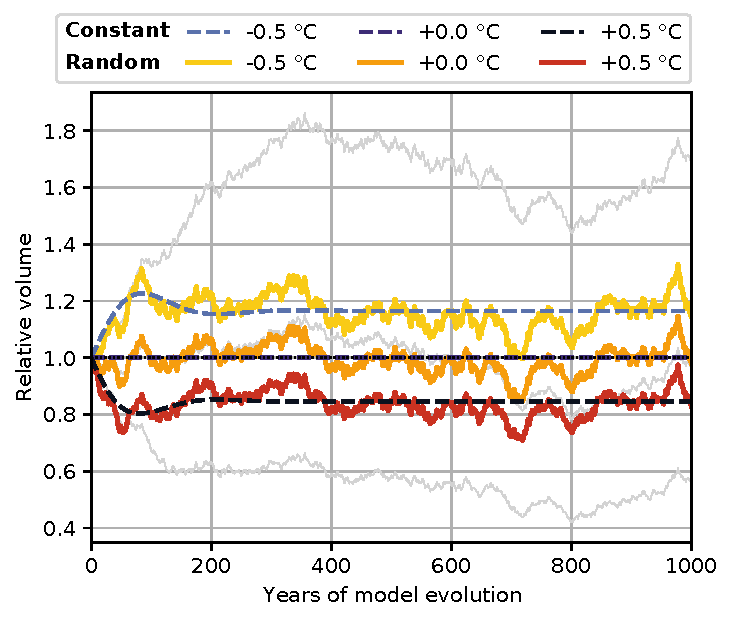
\includegraphics[width=\textwidth]{../plots/final_plots/time_series/single_glaciers/volume_norm_vas_Hintereisferner.pdf}
          \end{subfigure}
          \hfill
          % Flowline volume
          \begin{subfigure}[b]{0.476\textwidth}
            \caption{Flowline model, relative ice volume}
            \label{fig:hintereisferner:volume_fl}
            \centering
            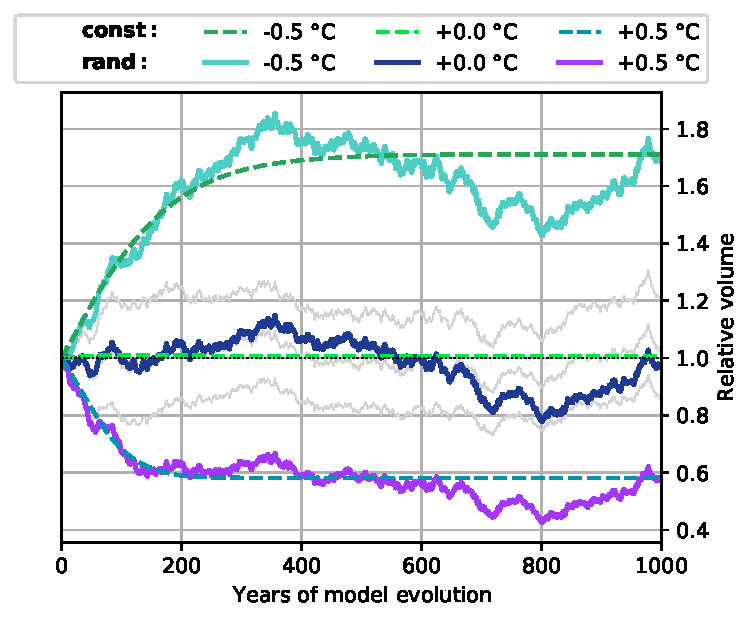
\includegraphics[width=\textwidth]{../plots/final_plots/time_series/single_glaciers/volume_norm_fl_Hintereisferner.pdf}
          \end{subfigure}
          % VAS area
          \begin{subfigure}[b]{0.476\textwidth}
            \caption{\Vas{} model, relative surface area}
            \label{fig:hintereisferner:area_vas}
            \centering
            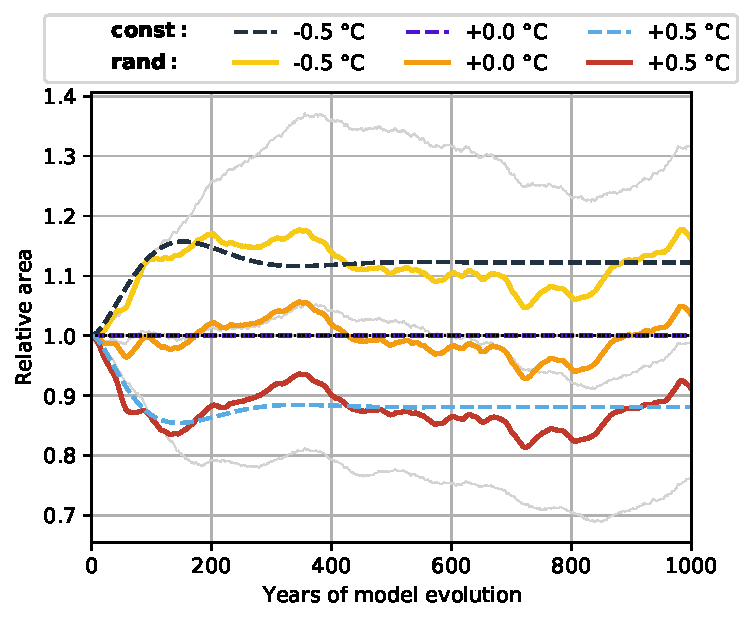
\includegraphics[width=\textwidth]{../plots/final_plots/time_series/single_glaciers/area_norm_vas_Hintereisferner.pdf}
          \end{subfigure}
          \hfill
          % Flowline area
          \begin{subfigure}[b]{0.476\textwidth}
            \caption{Flowline model, relative surface area}
            \label{fig:hintereisferner:area_fl}
            \centering
            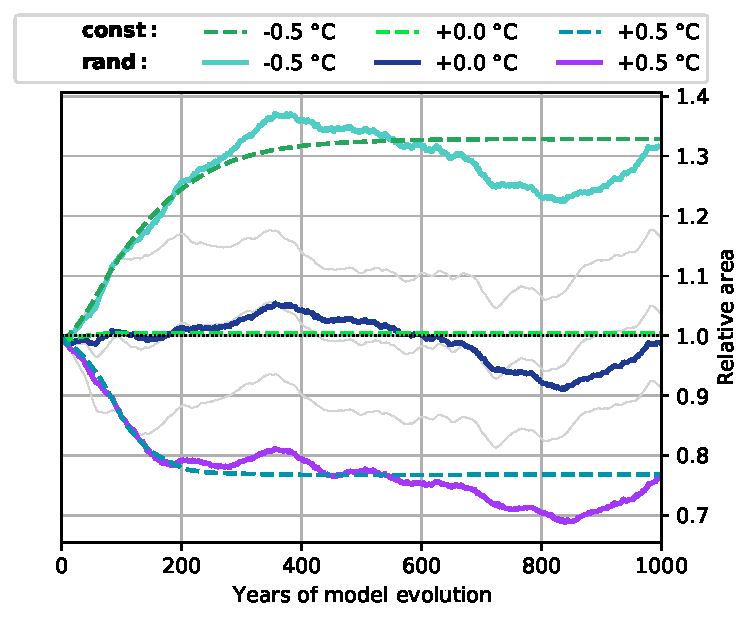
\includegraphics[width=\textwidth]{../plots/final_plots/time_series/single_glaciers/area_norm_fl_Hintereisferner.pdf}
          \end{subfigure}
          % VAS length
          \begin{subfigure}[b]{0.476\textwidth}
            \caption{\Vas{} model, relative glacier length}
            \label{fig:hintereisferner:length_vas}
            \centering
            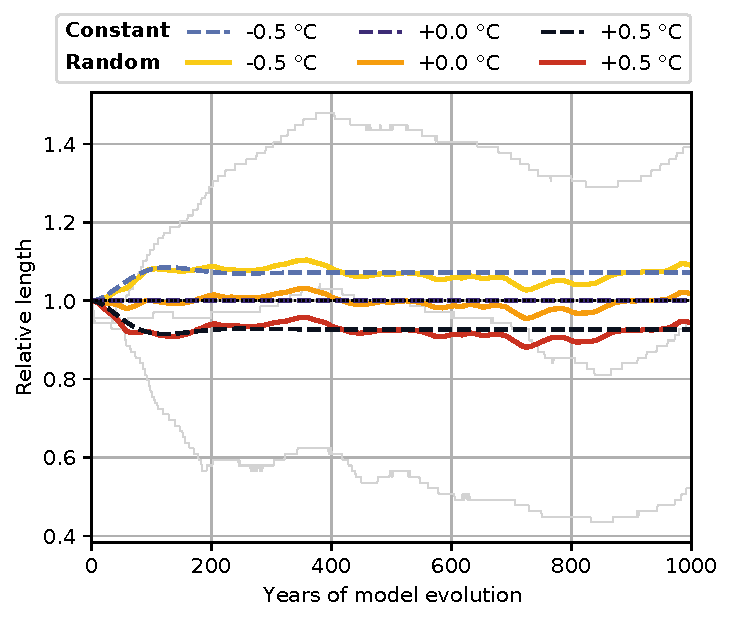
\includegraphics[width=\textwidth]{../plots/final_plots/time_series/single_glaciers/length_norm_vas_Hintereisferner.pdf}
          \end{subfigure}
          \hfill
          % Flowline length
          \begin{subfigure}[b]{0.476\textwidth}
            \caption{Flowline model, relative glacier length}
            \label{fig:hintereisferner:length_fl}
            \centering
            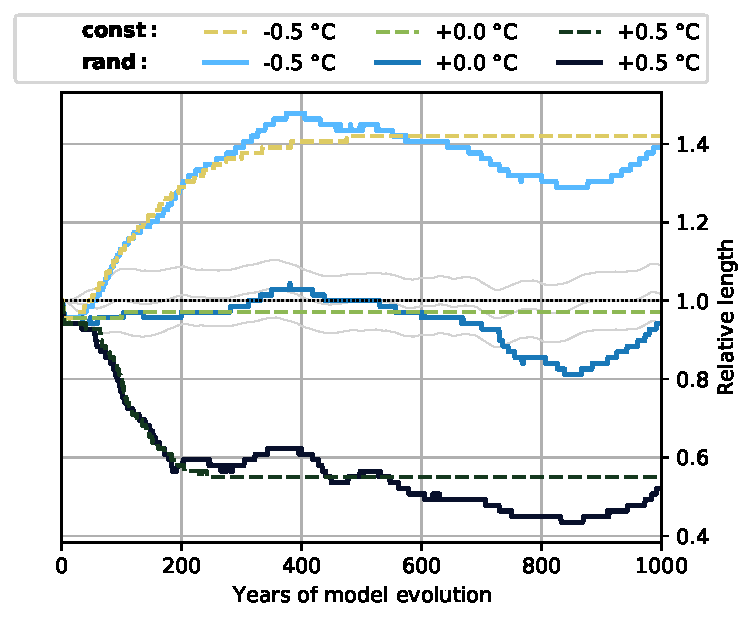
\includegraphics[width=\textwidth]{../plots/final_plots/time_series/single_glaciers/length_norm_fl_Hintereisferner.pdf}
          \end{subfigure}
          
          \caption{Temporal evolution of ice volume in (\subref{fig:hintereisferner:volume_vas}) and (\subref{fig:hintereisferner:volume_fl}), surface area in (\subref{fig:hintereisferner:area_vas}) and (\subref{fig:hintereisferner:area_fl}) and glacier length in (\subref{fig:hintereisferner:length_vas}) and (\subref{fig:hintereisferner:length_fl}) for Hintereisferner (RGI60-11.00897). The shown values area normalized with their respective initial values. The left panels show the result of the \vas{} model, the right panels show the results of the flowline model. Solid lines represent the random climate scenarios, while dashed lines represent the constant climate scenarios. All climate scenarios are based on an equilibrium climate. The applied temperature biases of \SI{-.5}{\celsius}, \SI{0}{\celsius} and \SI{+.5}{\celsius} are color coded, see legend for details. The dotted line indicates the initial volume. The light gray lines represent the volume evolutions of the other model, to facilitate comparisons.}
          \label{fig:hintereisferner}
        \end{figure}
      
      % subsubsection hintereisferner_test_case_results (end)

      \subsubsection{Commitment runs on a regional scale} % (fold)
      \label{ssub:commitment_runs_results}

        At the risk of repetition, \vas{} should not be applied to individual glaciers but to populations of glaciers \citep{Bahr2015}. This is were the scaling approach shows its strength. The law of large number assures a reasonable estimation of the collective glacier ice volume, since random error will be canceled out by each other. Hence, this section examines the behavior of \vas{} model applied to all Alpine glaciers. The findings explained hereafter result from runs under
        \begin{enumerate*}[label=(\alph*)]
          \item an equilibrium climate, with \lstinline`y0` = \tstar{} for each glacier
          \item todays climate, with \lstinline`y0 = 1999`
        \end{enumerate*}.
        Both climate scenarios run with different mass balance models and apply different temperature biases. For more details see Section~\ref{ssub:commitment_runs_setup}.

        Let's first take a more general look at the model behavior under equilibrium climate, similar to the Hintereisferner test case (Section~\ref{ssub:hintereisferner_test_case_results}. Both evolution models run for 1'000 years, once with the \lstinline`ConstantMassBalance` model and once with the \lstinline`RandomMassBalance` model. A random climate with its year-to-year fluctuations is obviously more physical than a completely constant climate. However, the changes in glacier ice volume under both climate scenarios are almost identical. Over the last 200 years of the simulations with equilibrium climate, the differences in total ice volume between the constant and random climate scenario average around \SI{0.6}{\percent} to \SI{0.7}{\percent} for the \vas{} model and \SI{0.7}{\percent} to \SI{2.3}{\percent} for the flowline model, depending on the temperature bias. This makes intuitive sense, considering that glaciers act as natural low-pass filters for climatic variabilities. For this reason and to simplify the following discussion, only the constant climate scenarios are investigated further.

        The \vas{} model estimates a total Alpine ice volume of \SI{139}{\cubic\kilo\meter} (\SI{+6}{\percent}), \SI{115}{\cubic\kilo\meter} (\SI{-12}{\percent}) and \SI{95}{\cubic\kilo\meter} (\SI{-27}{\percent}), while the flowline model estimates a total Alpine ice volume of \SI{236}{\cubic\kilo\meter} (\SI{+45}{\percent}), \SI{147}{\cubic\kilo\meter} (\SI{-10}{\percent}) and \SI{86}{\cubic\kilo\meter} (\SI{-47}{\percent}), for a temperature bias of \SI{-.5}{\celsius}, \SI{0}{\celsius} and \SI{+.5}{\celsius}, respectively. 
        Both evolution models adjust their initial ice volume downwards by under equilibrium climate. This is due to the mass balance residual \bias{}. It indicates that the 2003 RGI geometries are not sustainable by any 31-period in the HISTALP records \citep{Maussion2019}. This sag could be eliminated by a spin-up period, but since the absolute values are of less interest for now it seems unnecessary.
        As seen before, the \vas{} scaling model underestimates the change in ice volume compared to the flowline model.

        \begin{figure}[htp]
          \centering
          \begin{subfigure}[b]{0.48\textwidth}
            \caption{\Vas{} model, relative glacier volume}
            \label{fig:histalp_commitment:volume_norm_const}
            \centering
            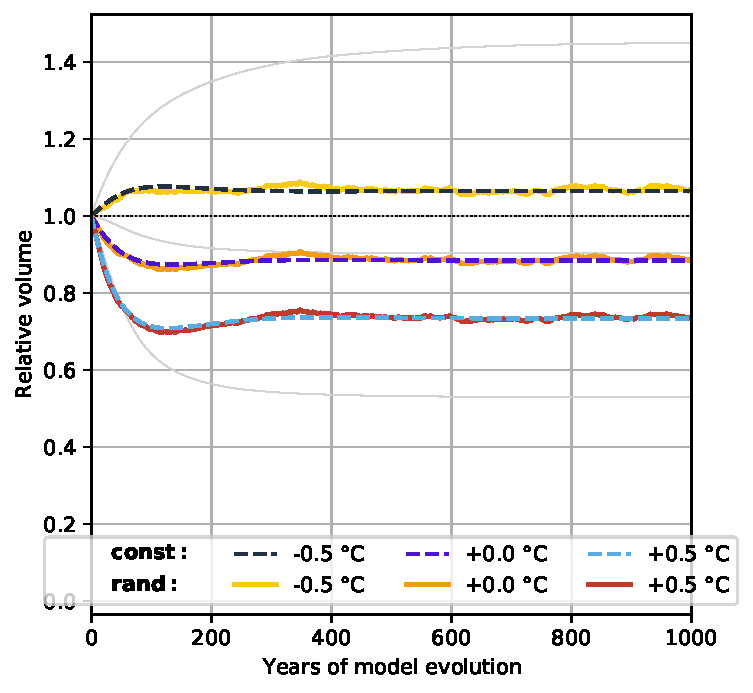
\includegraphics[width=\textwidth]{../plots/final_plots/time_series/histalp_commitment/volume_norm_vas.pdf}
          \end{subfigure}
          \hfill
          \begin{subfigure}[b]{0.48\textwidth}
            \caption{Flowline model, relative glacier volume}
            \label{fig:histalp_commitment:volume_norm_random}
            \centering
            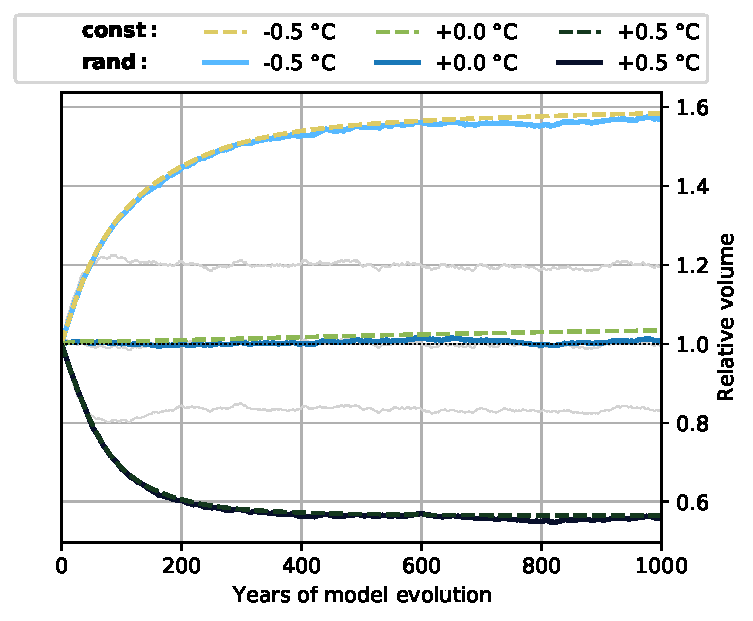
\includegraphics[width=\textwidth]{../plots/final_plots/time_series/histalp_commitment/volume_norm_fl.pdf}
          \end{subfigure}
          \begin{subfigure}[b]{0.48\textwidth}
            \caption{\Vas{} model, absolute glacier volume}
            \label{fig:histalp_commitment:volume_abs_const}
            \centering
            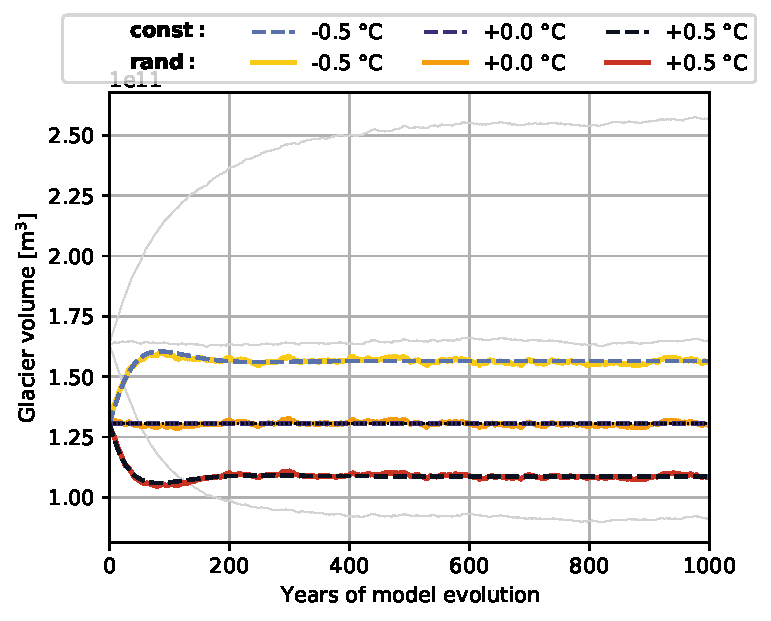
\includegraphics[width=\textwidth]{../plots/final_plots/time_series/histalp_commitment/volume_abs_vas.pdf}
          \end{subfigure}
          \hfill
          \begin{subfigure}[b]{0.48\textwidth}
            \caption{Flowline model, absolute glacier volume}
            \label{fig:histalp_commitment:volume_abs_random}
            \centering
            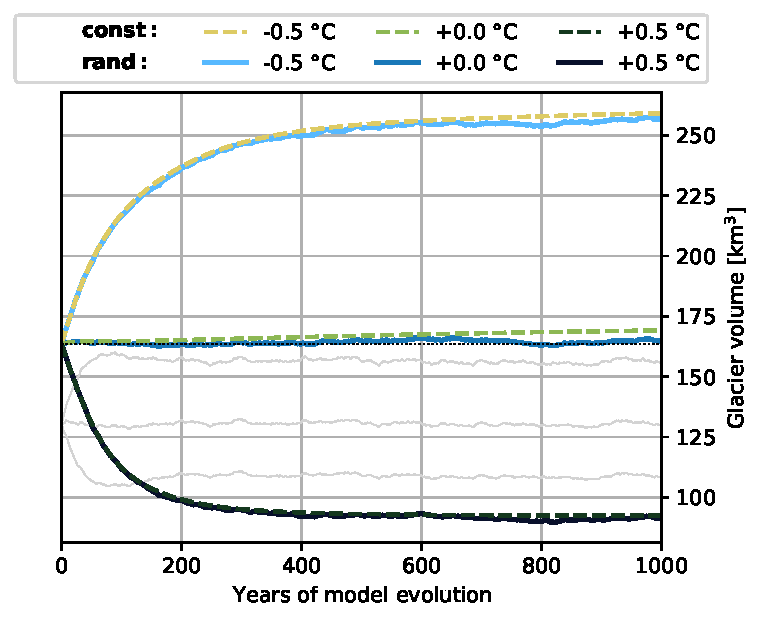
\includegraphics[width=\textwidth]{../plots/final_plots/time_series/histalp_commitment/volume_abs_fl.pdf}
          \end{subfigure}
          
          \caption{Time series of total ice volume for all glaciers in the HISTALP domain. The upper two panels show the relative glacier ice volume, normalized with the initial values, while the lower two panels show the absolute glacier ice volume. The left panels show the result of the \vas{} model, the right panels show the results of the flowline model. Solid lines represent the random climate scenarios, while dashed lines represent the constant climate scenarios. All climate scenarios are based on an equilibrium climate, with one of three different temperature biases.
          Yellow, orange and red solid lines represent the \vas{} model, while cyan, blue and purple solid lines represent the flowline model, under a random climate with a temperature bias of \SI{-.5}{\celsius}, \SI{0}{\celsius} and \SI{+.5}{\celsius}, respectively. Yellow, orange and red dashed lines represent the \vas{} model, while cyan, blue and purple dashed lines represent the flowline model, under a constant climate with a temperature bias of \SI{-.5}{\celsius}, \SI{0}{\celsius} and \SI{+.5}{\celsius}, respectively. %TODO change colors
          The dotted line indicate the initial volume. The light gray lines represent the volume evolutions of the other model, to facilitate comparisons.}
          \label{fig:histalp_commitment}
        \end{figure}

        % \begin{figure}[htp]
        %   \centering
        %   \begin{subfigure}[b]{0.99\textwidth}
        %     \caption{Normalized glacier volume}
        %     \label{fig:histalp_commitment:volume_norm}
        %     \centering
        %     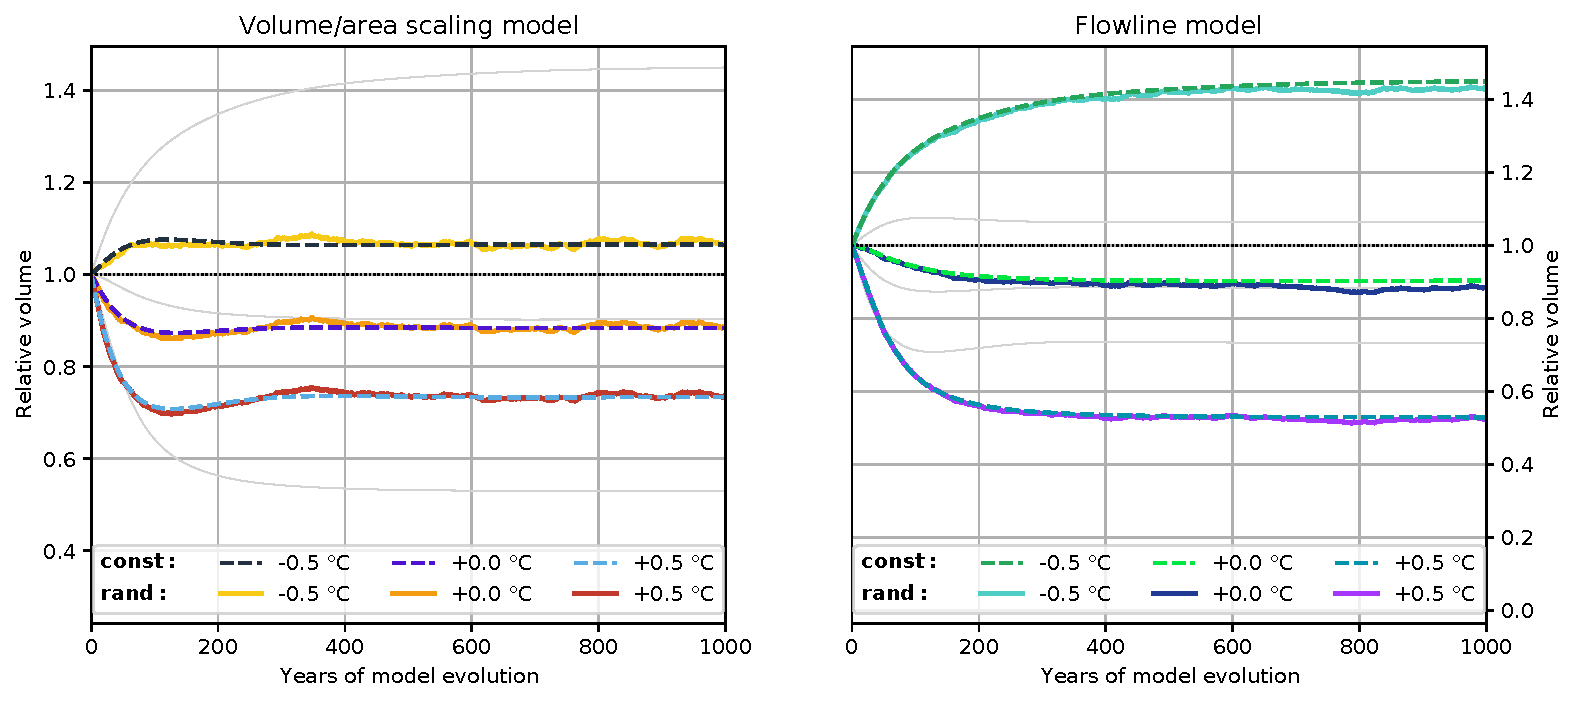
\includegraphics[width=\textwidth]{../plots/final_plots/time_series/histalp_commitment/volume_norm.pdf}
        %   \end{subfigure}
        %   \begin{subfigure}[b]{0.99\textwidth}
        %     \caption{Absolute glacier volume}
        %     \label{fig:histalp_commitment:volume_abs}
        %     \centering
        %     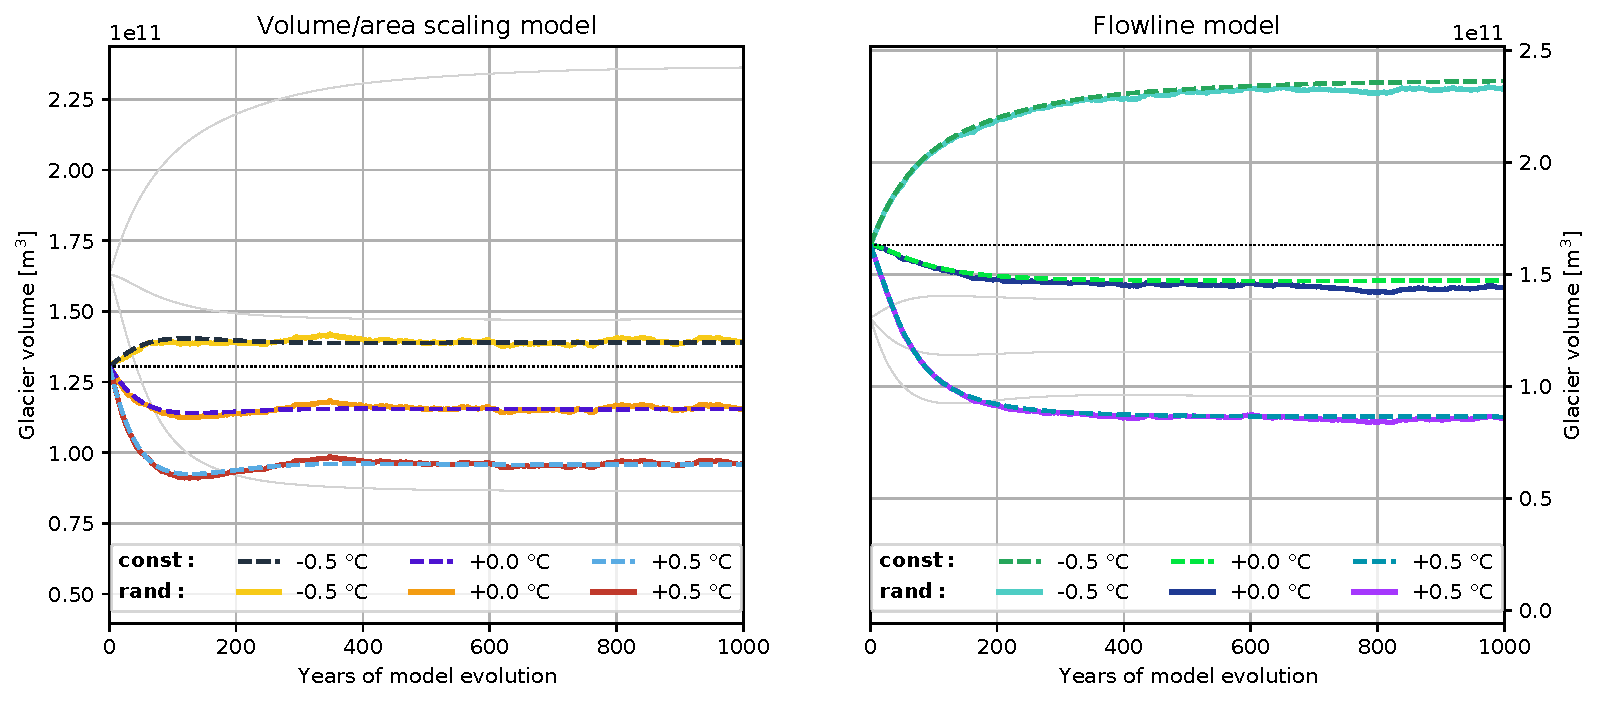
\includegraphics[width=\textwidth]{../plots/final_plots/time_series/histalp_commitment/volume_abs.pdf}
        %   \end{subfigure}
          
        %   \caption{Time series of total ice volume for all glaciers in the HISTALP domain. The upper two panels show the relative values, normalized with the initial values, while the lower two panels show absolute values. The left panels show the result of the \vas{} model, the right panels show the results of the flowline model. Solid lines represent a random climate scenario, while dashed lines represent a constant climate scenario. All climate scenarios are based on an equilibrium climate, however with three different temperature biases.
        %   Yellow, orange and red solid lines represent the \vas{} model, while cyan, blue and purple solid lines represent the flowline model, under a random climate with a temperature bias of \SI{-.5}{\celsius}, \SI{0}{\celsius} and \SI{+.5}{\celsius}, respectively. Yellow, orange and red dashed lines represent the \vas{} model, while cyan, blue and purple dashed lines represent the flowline model, under a constant climate with a temperature bias of \SI{-.5}{\celsius}, \SI{0}{\celsius} and \SI{+.5}{\celsius}, respectively. %TODO change colors
        %   The dotted line indicate the initial volume. The light gray lines represent the volume evolutions of the other model, to facilitate comparisons.}
        %   \label{fig:histalp_commitment}
        % \end{figure}

      % subsubsection commitment_runs_results (end)

    % subsection time_series (end)

    \subsection{Autocorrelation analysis} % (fold)
    \label{sub:autocorrelation_analysis_results}

      The autocorrelation function for selected glaciers is shown in Figure~\ref{fig:acf}. For details about the experimental setup see Section~\ref{ssub:autocorrelation_analysis_setup}

      The autocorrelation function of the \vas{} length shows little to no variability between runs under different climate conditions. % TODO compare with almost linear behavior of mass balance model in the vicinity of equilibirum
      The autocorrelation function of the \vas{} length is comparable even between different glaciers. It has the same behavior of a dampened oscillator as described above. Their are differences in amplitude and frequency--most likely affected by size--the general behavior is almost identical. 
      
      The flowline model is able to represent different glacial geometries and grasp individual responses to climatic forcings, which can be seen in the vastly different autocorrelation functions. They differ from to glacier, but also for different climate scenarios (temperature biases) on the same glacier. However, there are no discernible patterns, which again confirms the notion that the OGGM flowline model is capable of modeling each glaciers individual response. Here are some examples: for Hintereisferner the autocorrelation of the flowline model is stronger than that of the \vas{} model, while for Mer de Glace and Großer Aletschgletscher it is lower (for all tested climate scenarios); the flowline model of the Pasterze shows a strong autocorrelation under the equilibrium climate, i.e., \SI{0}{\celsius} temperature bias, (>0.7 for lags times between 0 and 95 years, still >0.43 for 200 years lag time, statistically significant up until a lag time of 232 years), while with a positive and negative temperature bias of \SI{\pm0.5}{\celsius} the autocorrelation is less than for the \vas{} model.
      The \vas{} model has a stronger autocorrelation for short lag time (i.e., less than about 20 years) than the flowline model; similarly, the flowline model of the d'Argentière shows a strong autocorrelation under the climate with \SI{+0.5}{\celsius} temperature bias, and lower autocorrelation than the \vas{} model for the other two climate scenarios; The only observation made for all glaciers, it that the \vas{} model has a stronger autocorrelation for short lag time (i.e., less than about 20 years) than the flowline model. This is true even for glaciers, where the autocorrelation of the flowline mode is generally stronger (e.g., Hintereisferner). 

      It is not the intent of this work to investigate the relation between a glacier's geometry and its autocorrelation function, therefore we leave it at this qualitative first look. However, it is notable that the OGGM flowline model behaves differently for different glaciers and/or different climatic forcings. How far these results are comparable to real world glaciers is anyones guess. The \textit{one size fits all} approach of the \vas{} model produces comparable results, mostly independent the glaciers geometry and the climate forcing (which was to be expected).


      \begin{figure}[htp]
        \centering
        \begin{subfigure}[b]{0.48\textwidth}
          \caption{RGI60-11.00897 - Hintereisferner}
          \label{fig:acf:hintereisferner}
          \centering
          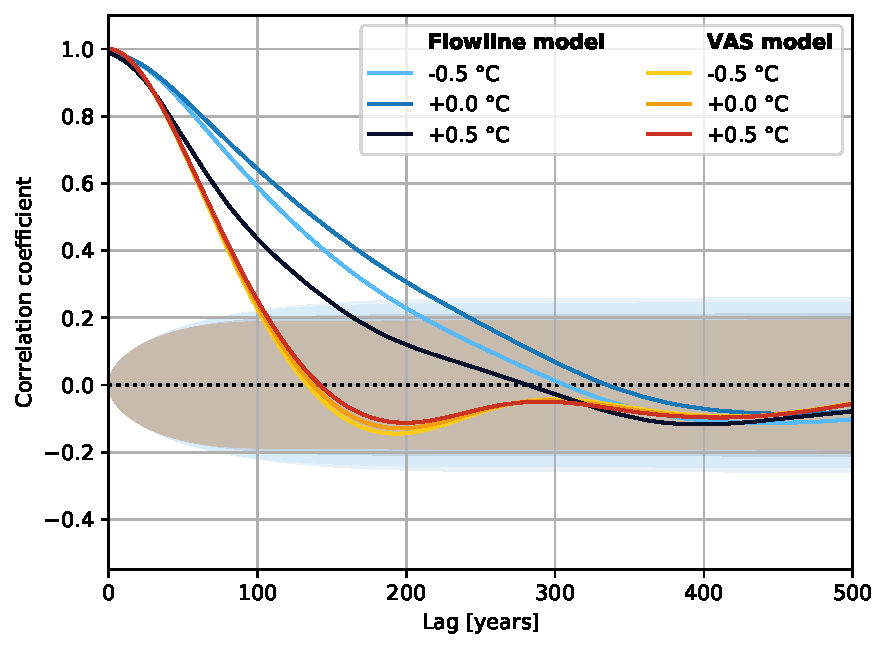
\includegraphics[width=\textwidth]{../plots/final_plots/acf/Hintereisferner.pdf}
        \end{subfigure}
        \hfill
        \begin{subfigure}[b]{0.48\textwidth}
          \caption{RGI60-11.00106 - Pasterze}
          \label{fig:acf:pasterze}
          \centering
          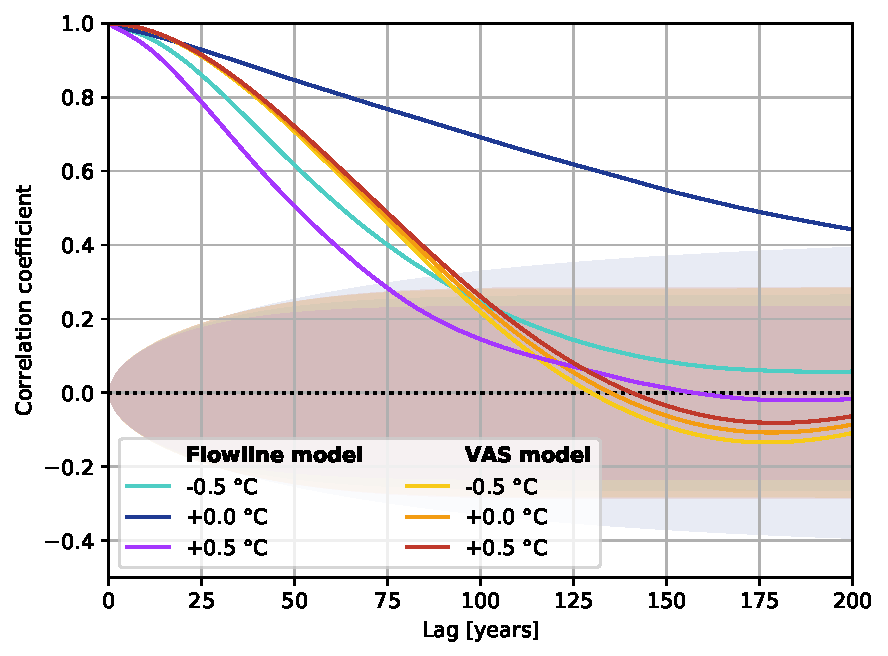
\includegraphics[width=\textwidth]{../plots/final_plots/acf/Pasterze.pdf}
        \end{subfigure}
        \begin{subfigure}[b]{0.48\textwidth}
          \caption{RGI60-11.03643 - Mer de Glace}
          \label{fig:acf:mer_de_glace}
          \centering
          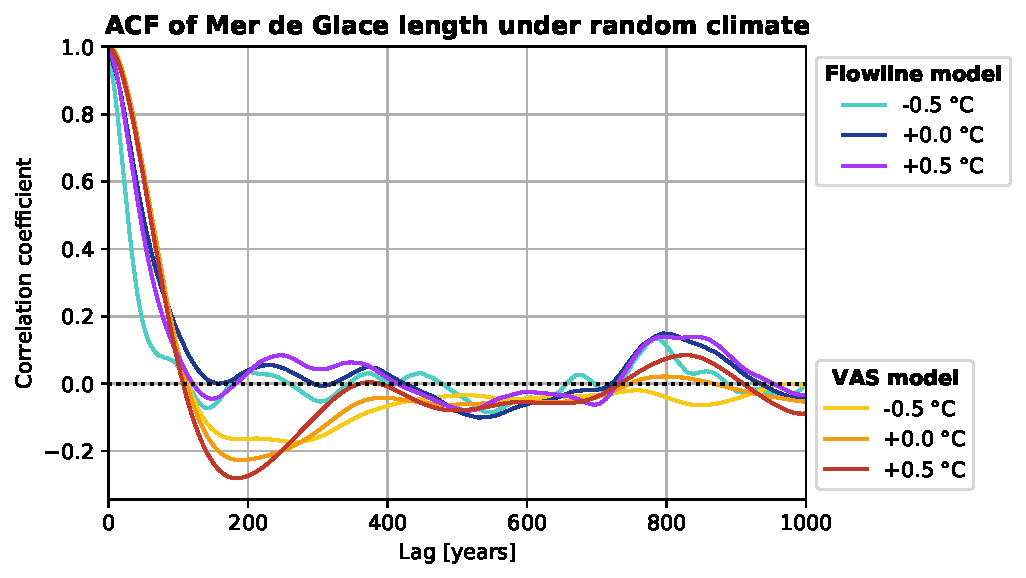
\includegraphics[width=\textwidth]{../plots/final_plots/acf/Mer_de_Glace.pdf}
        \end{subfigure}
        \hfill
        \begin{subfigure}[b]{0.48\textwidth}
          \caption{RGI60-11.03638 - d'Argentière}
          \label{fig:acf:glacier_d_argentiere}
          \centering
          \includegraphics[width=\textwidth]{../plots/final_plots/acf/Glacier_d'Argentière.pdf}
        \end{subfigure}
        \begin{subfigure}[b]{0.48\textwidth}
          \caption{RGI60-11.01450 - Großer Aletschgletscher}
          \label{fig:acf:großer_aletschgletscher}
          \centering
          \includegraphics[width=\textwidth]{../plots/final_plots/acf/Großer_Aletschgletscher.pdf}
        \end{subfigure}
        \hfill
        \begin{subfigure}[b]{0.48\textwidth}
          \caption{RGI60-11.01238 - Rhonegletscher}
          \label{fig:acf:rhonegletscher}
          \centering
          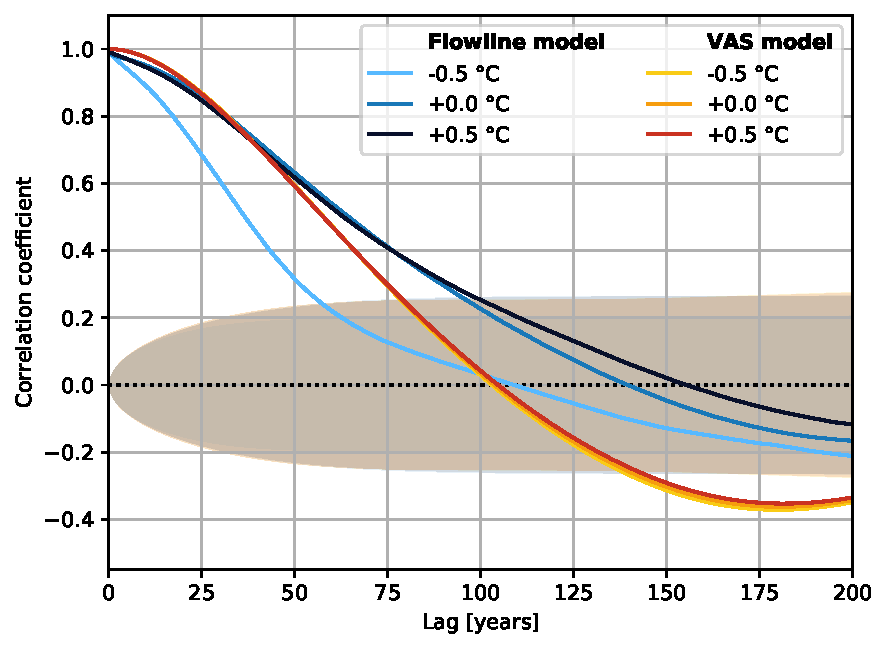
\includegraphics[width=\textwidth]{../plots/final_plots/acf/Rhonegletscher.pdf}
        \end{subfigure}
        % \begin{subfigure}[b]{0.48\textwidth}
        %   \caption{RGI60-11.02704 - Allalingletscher}
        %   \label{fig:acf:allalingletscher}
        %   \centering
        %   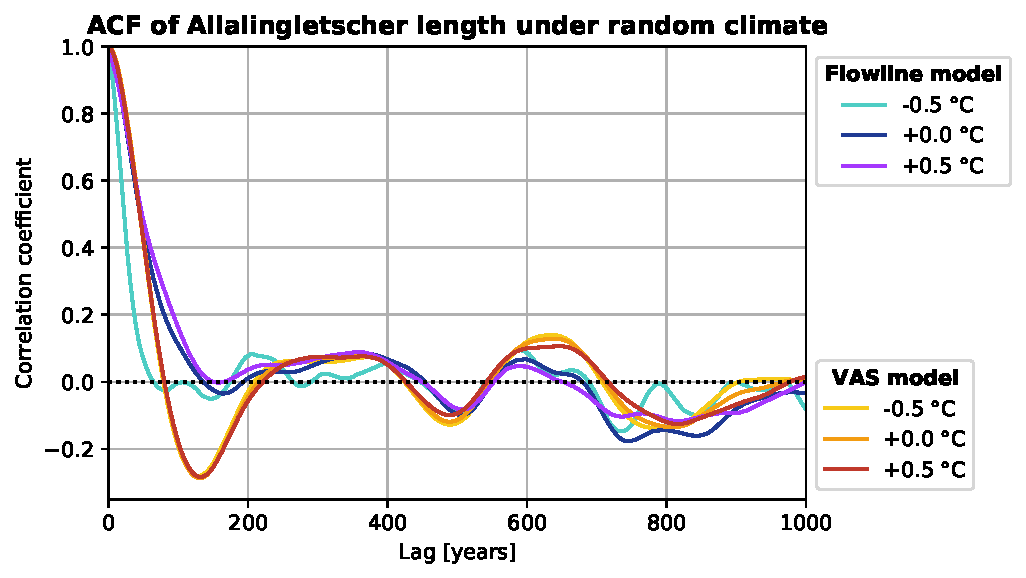
\includegraphics[width=\textwidth]{../plots/final_plots/acf/Allalingletscher.pdf}
        % \end{subfigure}
        % \hfill
        % \begin{subfigure}[b]{0.48\textwidth}
        %   \caption{RGI60-11.02773 - Findelgletscher}
        %   \label{fig:acf:findelgletscher}
        %   \centering
        %   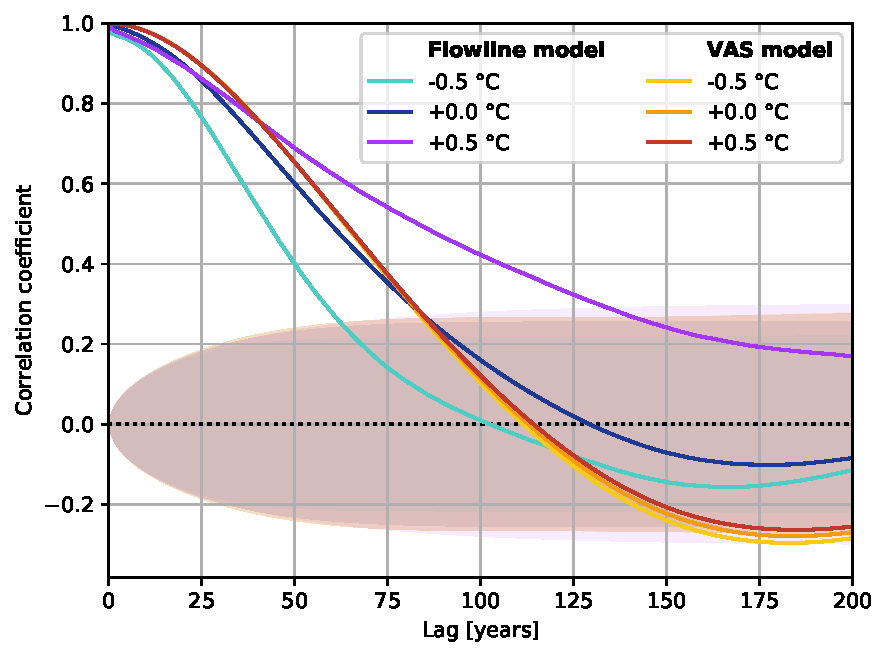
\includegraphics[width=\textwidth]{../plots/final_plots/acf/Findelgletscher.pdf}
        % \end{subfigure}

        \caption{Autocorrelation function of modeled length for lag times between zero and 200 years. Different lines represent different combinations of evolution model and climate scenario.
        The random climate scenario is based on an equilibrium climate, with different temperature biases.
        Cyan, blue and purple lines represent the flowline model, while yellow, orange and red lines represent the \vas{} model, with a temperature bias of \SI{-.5}{\celsius}, \SI{0}{\celsius} and \SI{+.5}{\celsius}, respectively.
        The \SI{99}{\percent} confidence intervals are shaded in the corresponding colors.}
        \label{fig:acf}
      \end{figure}
    
    % subsection sub:autocorrelation_analysis_results (end)

    \subsubsection{Power spectral density analysis} % (fold)
    \label{ssub:power_spectral_density_analysis}
    
    % subsubsection power_spectral_density_analysis (end)

% section equilibrium_experiments (end)

% ==== SECTION 2 ===============================================================
\section{Sensitivity experiments} % (fold)
\label{sec:sensitivity_experiments_results}

% section sensitivity_experiments (end)

% ==== SECTION 3 ===============================================================
\section{Future projection} % (fold)
\label{sec:future_projection_results}

% section future_projection (end)